% =====================================================================
%  Synthetic "dimpled sphere" dataset — thesis section
%  Requires: amsmath, graphicx, booktabs.  (siunitx optional; units here are plain text.)
%  Generated by:  scripts/generate_dimpled_object.py
%  Figures by:     scripts/figure_dataset_depths.py, figure_dataset_residual.py, figure_camera_rig.py
%  Adjust the \graphicspath / figure paths to wherever you copy figures/.
% =====================================================================

\section{Synthetic Evaluation Dataset}
\label{sec:dataset}

To evaluate the depth-fusion stage in isolation we use a controlled synthetic object, the
\emph{dimpled sphere}. It is deliberately designed so that the silhouette-based visual hull can
recover the body almost perfectly, while the surface detail is \emph{concave} and therefore invisible
to silhouettes: any error in those concavities can be attributed to the depth fusion alone. The object,
the ground-truth mesh, the camera calibration, and the depth maps are all produced analytically and
\emph{without sensor noise}, so every reconstruction error reported in this chapter is systematic
rather than a property of a particular sensor.

\subsection{Object definition}
\label{sec:dataset-object}

The object is the Boolean difference of a base sphere and several smaller ``pocket'' spheres,
expressed directly as a signed distance field (SDF) $f(\mathbf{p})$ that is negative inside the solid.
A spherical pocket is removed with the standard constructive-solid-geometry difference operator
$A \setminus B = \max(A, -B)$, giving
%
\\begin{equation}
  f(\mathbf{p}) \;=\;
  \max\!\Bigl(\;
    \underbrace{\lVert\mathbf{p}\rVert - R}_{\text{base sphere}},\;\;
    \max_{k=1}^{K}\bigl(r_{p} - \lVert\mathbf{p}-\mathbf{c}_{k}\rVert\bigr)
  \Bigr),
  \label{eq:dimpled-sdf}
\end{equation}
%
with base radius $R = 0.5\,\text{m}$ and $K = 12$ pockets of radius $r_{p} = 0.19\,\text{m}$. The
pocket centres $\mathbf{c}_{k}$ are placed on Fibonacci-sphere directions at radius
$R + \delta = 0.60\,\text{m}$, i.e.\ just \emph{outside} the surface, so that each pocket carves a
shallow spherical-cap bowl approximately $0.09\,\text{m}$ deep into the sphere. Because the pockets
point in all directions, every viewing direction exposes a different subset of them, which is what
makes the number of depth cameras a meaningful variable. As the geometry is an SDF, both the ground
truth and the depth maps are derived from the \emph{same} analytic function, eliminating any
mesh-versus-render mismatch.

\subsection{Ground-truth mesh}
\label{sec:dataset-gt}

The reference surface is obtained by sampling $f$ on a $256^{3}$ grid over $[-0.75, 0.75]^{3}\,\text{m}$
and triangulating the zero level set with marching cubes; the resulting voxel coordinates are mapped
back to world units. This yields a watertight mesh of roughly $143{,}000$ vertices, against which all
Chamfer and region-split metrics are computed.

\subsection{Camera configuration}
\label{sec:dataset-cameras}

All cameras are ideal pinhole cameras looking at the origin, with focal length
$f_{x} = f_{y} = 1400\,\text{px}$, a centred principal point, and a resolution of
$1920 \times 1080$. Two camera sets are used:
%
\begin{itemize}
  \item \textbf{RGB cameras} ($60$, fixed for every experiment): placed on a Fibonacci sphere of
    radius $2.5\,\text{m}$ for dense, isotropic silhouette coverage, giving a constant and well-formed
    visual hull across all runs.
  \item \textbf{Depth cameras} ($N$, swept from $1$ to $30$): placed by greedy farthest-point sampling
    over a dense Fibonacci candidate set at radius $2.5\,\text{m}$. Because the greedy order is
    deterministic, the first $N$ positions are a prefix of the first $M>N$: adding a depth camera
    \emph{keeps} all previous ones and only appends new, maximally separated viewpoints. The
    camera-count sweep is therefore strictly additive (``add a camera'', not ``re-arrange $N$
    cameras''). The full $30$-camera rig is shown in Figure~\ref{fig:camera-rig}.
\end{itemize}

\subsection{Rendering}
\label{sec:dataset-rendering}

\paragraph{Silhouette masks.} A pixel belongs to the object iff its ray intersects the base sphere,
determined analytically from the sign of the ray--sphere discriminant. The pockets are intentionally
absent from the silhouette, since a concavity cannot change an object's outline; consequently the RGB
visual hull is exactly the smooth sphere.

\paragraph{Depth maps.} Depth is rendered with a sphere-tracing-style SDF surface finder. Only rays
inside the silhouette are marched, over the sphere's entry--exit interval in $256$ fixed steps; the
first sign change of $f$ along a ray marks the surface hit, and the along-ray hit distance is converted
to an optical-axis depth. Pixels without a hit receive a constant background depth of $5.0\,\text{m}$.
The pockets appear as the deeper (farther) patches on the sphere face, as illustrated in
Figures~\ref{fig:dataset-depth} and~\ref{fig:dataset-residual}. Depth is stored as a 16-bit image in
millimetres.

\subsection{Parameter summary}
\label{sec:dataset-params}

\begin{table}[ht]
  \centering
  \begin{tabular}{ll}
    \toprule
    Parameter & Value \\
    \midrule
    Base sphere radius $R$                    & $0.50\,\text{m}$ \\
    Number of pockets $K$                     & $12$ (Fibonacci-distributed) \\
    Pocket radius $r_p$ / centre offset $\delta$ / depth & $0.19\,\text{m}$ / $0.10\,\text{m}$ / $\approx 0.09\,\text{m}$ \\
    RGB cameras                               & $60$, Fibonacci sphere, $r = 2.5\,\text{m}$ \\
    Depth cameras                             & $1$--$30$, nested farthest-point, $r = 2.5\,\text{m}$ \\
    Intrinsics                                & $f_x = f_y = 1400\,\text{px}$, $1920\times1080$, centred \\
    Ground-truth extraction                   & $256^{3}$ SDF grid on $[-0.75,0.75]\,\text{m}$, marching cubes \\
    Depth rendering                           & $256$-step SDF root find, $5.0\,\text{m}$ background, noise-free \\
    \bottomrule
  \end{tabular}
  \caption{Parameters of the synthetic dimpled-sphere dataset.}
  \label{tab:dataset-params}
\end{table}

% --------------------------------------------------------------------
%  Figures (adjust paths to your figure directory)
% --------------------------------------------------------------------
\begin{figure}[ht]
  \centering
  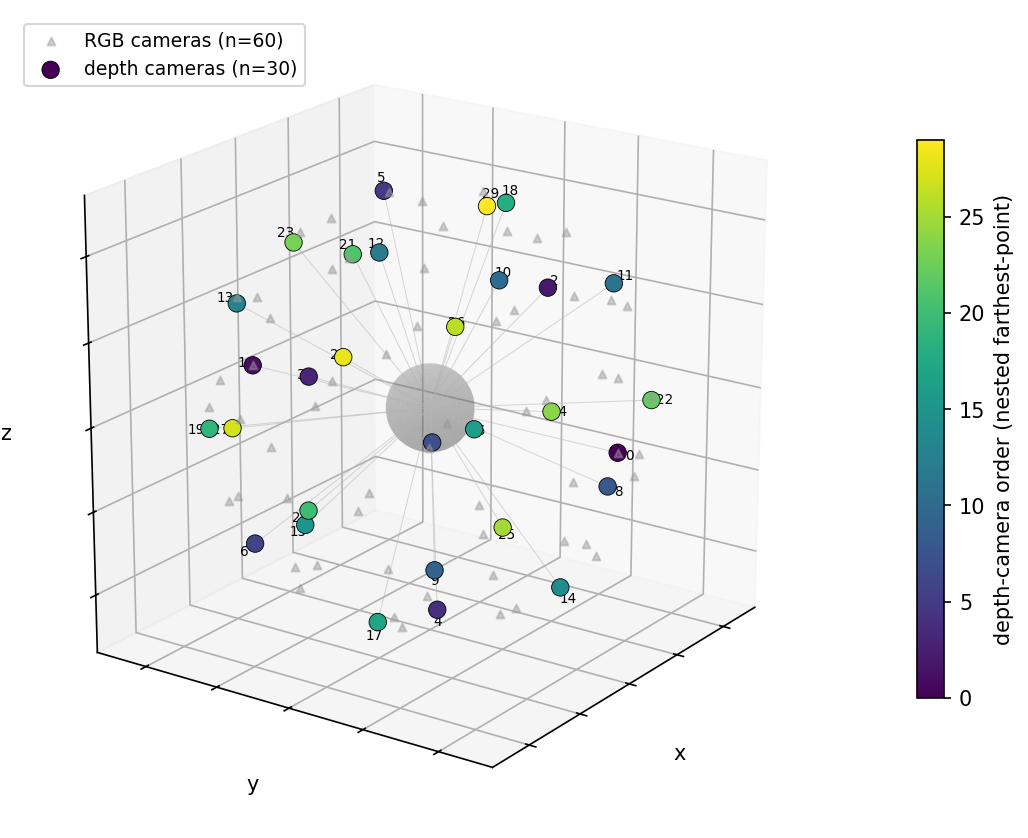
\includegraphics[width=\linewidth]{figures/06_camera_rig.png}
  \caption{Camera rig: the $30$ depth cameras (coloured by their nested farthest-point order) and the
    $60$ fixed RGB cameras, all at radius $2.5\,\text{m}$ and oriented towards the object at the origin.}
  \label{fig:camera-rig}
\end{figure}

\begin{figure}[ht]
  \centering
  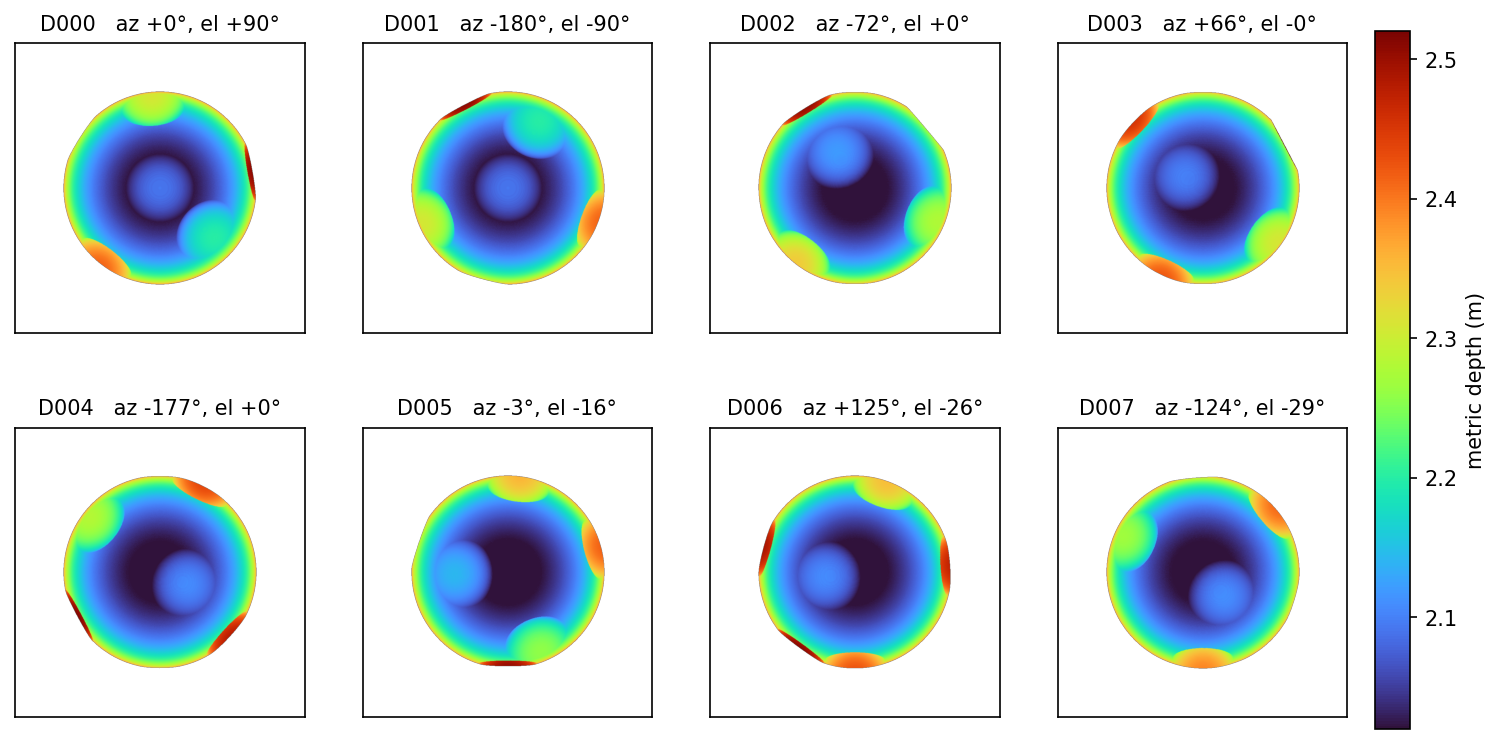
\includegraphics[width=\linewidth]{figures/05_dataset_depth_views.png}
  \caption{Ray-marched depth maps of the dimpled sphere from eight of the thirty depth cameras
    (azimuth/elevation indicated). The pockets appear as the deeper patches; the background is masked.}
  \label{fig:dataset-depth}
\end{figure}

\begin{figure}[ht]
  \centering
  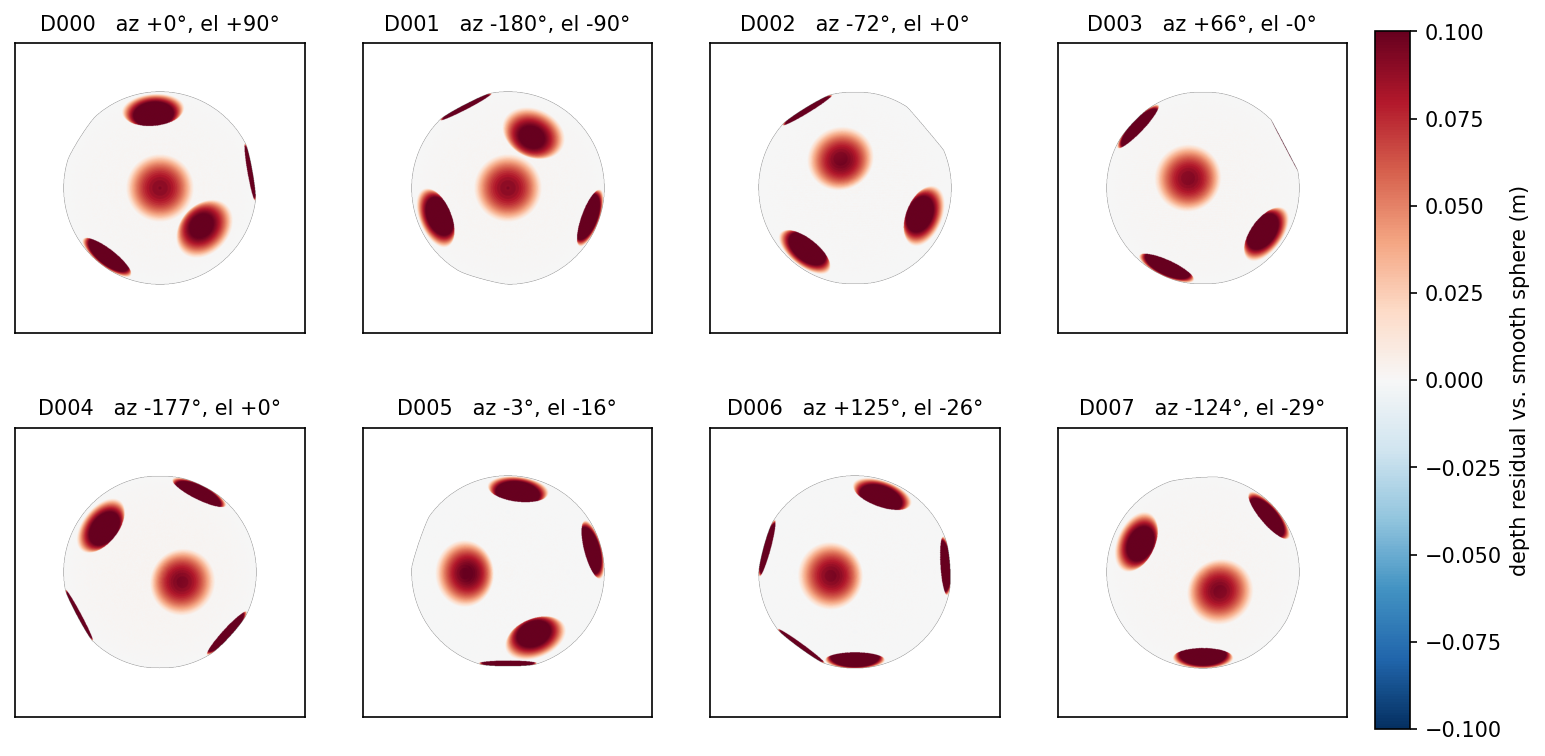
\includegraphics[width=\linewidth]{figures/05b_dataset_pocket_residual.png}
  \caption{The same views with the analytic smooth-sphere depth subtracted, removing the sphere's own
    curvature. The twelve concave pockets stand out as the recessed (red) bowls -- the surface detail
    that only depth can reconstruct.}
  \label{fig:dataset-residual}
\end{figure}
1